\chapter{Introduction}
\label{ch:graphcon::intro}


\begin{preamble}[Overview]
\label{graphcon::intro::motivate}
In earlier chapters, we have mostly covered techniques for solving
problems on graphs that were developed in the context of sequential
algorithms.  
%
Some of the algorithms we considered were parallel while others were
not.  For example, we saw that 
%
\href{ch:graphs::bfs}{BFS}
%
has some parallelism since each
level can be explored in parallel 
%
but there was no parallelism in
%
\href{ch:graphs::dfs}{DFS}.
%
There was no parallelism in
%
\href{ch:shortest-paths:dijkstra}{Dijkstra's algorithm},
%
but there was plenty of parallelism in the 
\href{ch:shortest-paths::bellman-ford}{Bellman-Ford algorithm}
and
\href{ch:shortest-paths::johnson}{Johnson's algorithm}.

In this part of the book, we cover the ``graph contraction'' technique.
%
This technique was specifically designed to be used in parallel
algorithms and allows obtaining poly-logarithmic span for certain
graph problems.
%
This chapter presents an overview of graph contraction.
%
The following chapters present two specializations
%
\href{ch:graphcon::edge}{Edge Contraction}
%
and
%
\href{ch:graphcon::star}{Star Contraction} of graph contraction,
%
and apply the technique to
%
\href{ch:graphcon::connect}{graph connectivity}.
% 
\end{preamble}



\section{Preliminaries}
\label{sec:graphcon::intro::prelim}


\begin{note}
\label{graphcon::intro::prelim::terminology}
The material here and the followup chapters on graph contraction relies on the graph terminology introduced in the background
%
\href{ch:bg::graphs}{chapter on graph theory}.
%
\end{note}

%% We review here the definition of graph partition.
%% %
%% Recall that a partition of a set $A$ is a set $P$ of non-empty subsets
%% of $A$ such that each element of $A$ is in exactly one subset $B \in
%% P$; each susbet $B \in P$ is called a~\defn{part} or~\defn{block.}
%% %
%% One important concept used in this chapter is the notion of graph
%% partition, which is a collection of graphs defined as vertex-induced
%% graphs of a set partition of its vertices.
%% \end{note}

\begin{definition}[Graph Partition]
\label{def:graphcon::intro::prelim::graph-partition}
Given a graph $G$, 
%
a~\defn{graph partition} of $G$ is a collection of graphs
%
\[
H_0 = (V_0, E_0), \ldots, H_{k-1} = (V_{k-1}, E_{k-1}),
\]
%
such that 
%
% $\bigcup_{i=0}{V_i} =V$, $\forall i. 0 \le i,j < k, V_i \not= \emptyset$
% and  $i \not= j \implies V_i \cap V_j = \emptyset$, 
%
$\{V_0, \ldots, V_{k-1}\}$ is a set partition of $V$
and 
%
$H_0, \ldots, H_{k-1}$ 
%
are 
%
\href{def:bg::graphs::subgraph::vi}{vertex-induced subgraphs}
%
of $G$ with respect to $V_0, \ldots, V_{k-1}$.
%

We refer to each subgraph $H_i$ as a~\defn{block} or~\defn{part} of~$G$.
\end{definition}
%


\begin{definition}[Internal and Cut Edges]
\label{def:graphcon::intro::prelim::edges}
Given a partition $H_0 = (V_0, E_0), \ldots, H_{k-1} = (V_{k_1}, E_{k-1})$
of a graph $G = (V, E)$,
%
we define two kinds of edges: internal edges and cut edges.
%

\begin{itemize}

\item

We call an edge $\{v_1,v_2\}$ an~\defn{internal edge}, if $v_1\in V_i$
and $v_2 \in V_i$.
%
Note that $\{v_1, v_2\} \in E_i$.
%

\item
We call an edge $\{v_1, v_2\}$ a~\defn{cut edge}, if $v_1\in V_i$
and $v_2 \in V_j$  and $i \not= j$.
%
\end{itemize}

\end{definition}


\begin{flex}
\begin{exercise}
One way to partition a graph is to make each connected component a
block. What are the internal and cut edges in such a partition?
\end{exercise}
\begin{solution}
There are no cut edges between the partitions. 
%
All edges of the graph are internal edges.
\end{solution}
\end{flex}

\begin{flex}
\begin{definition}[Partition Map]
\label{def:graphcon::intro::prelim::partition-map}
We sometimes describe a graph partition with a tuple consisting of 
%
\begin{enumerate}
\item a set of labels for the blocks, and 
\item a~\defn{partition map} that maps each vertex to the label of its
  block.
\end{enumerate}
%
The labels can be chosen arbitrarily but it is usually conceptually
and computationally easier to use a vertex inside a block as a
representative for that block.
%
\end{definition}

\begin{example}
\label{ex:graphcon::intro::prelim::partition-map}
The partition 
%
$\cset{\cset{\vname{a},\vname{b},\vname{c}},\cset{\vname{d}},\cset{\vname{e},\vname{f}}}$
%
of the vertices
%
$\cset{\vname{a},\vname{b},\vname{c},\vname{d},\vname{e},\vname{f}}$, 
%
defines three blocks as the corresponding 
%
\href{def:bg::graphs::subgraph::vi}{vertex-induced subgraphs}.

\begin{center}
  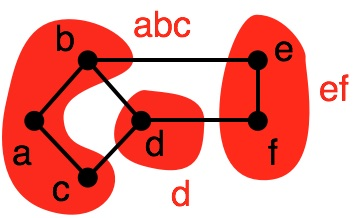
\includegraphics[width=2in]{./graph-contraction/media-introduction/contract-example3.jpg}
\end{center}
The edges $\cset{\vname{a},\vname{b}}$, $\cset{\vname{a},\vname{c}}$,
and $\cset{\vname{e},\vname{f}}$ are internal edges, and the edges
$\cset{\vname{c},\vname{d}}$, $\cset{\vname{b},\vname{d}}$,
$\cset{\vname{b},\vname{e}}$ and $\cset{\vname{d},\vname{f}}$ are
cut edges.

By labeling the blocks $\cstr{abc},\cstr{d}$ and
$\cstr{ef}$, we can specify the graph partition with following partition map:

\htmlmath{
\begin{alignat}{1}
( & \cset{\vname{abc}, \vname{d}, \vname{ef}},
\\
 & \cset{\vname{a} \mapsto
    \vname{abc}, \vname{b} \mapsto \vname{abc}, \vname{c} \mapsto
    \vname{abc}, \vname{d} \mapsto \vname{d}, \vname{e} \mapsto
    \vname{ef}, \vname{f} \mapsto \vname{ef}}
).
\end{alignat}
}

Instead of assigning a fresh label to each block, we can choose a
representative vertex.
%
For example, by picking $\vname{a}, \vname{d}$, and $\vname{e}$ as
representatives, we can represent the partition above using the
following partition map
\htmlmath{
\begin{alignat}{1}
( & \cset{\vname{a},\vname{d},\vname{e}}, 
\\
       & \cset{\vname{a} \mapsto \vname{a}, \vname{b} \mapsto \vname{a}, 
               \vname{c} \mapsto \vname{a}, \vname{d} \mapsto \vname{d}, 
               \vname{e} \mapsto \vname{e}, \vname{f} \mapsto
               \vname{e}}
).
\end{alignat}
}

\end{example}
\end{flex}

\section{Graph Contraction}
\label{ex:graphcon::intro::graphcon}

\begin{gram}
\label{graphcon::intro::graphcon::overview}
Graph contraction is a 
%
\href{ch:design::contraction}{contraction technique}
%
for computing properties of graphs in parallel.
%
As a contraction technique, it is used to solve a problem
instance by reducing it to a smaller instance of the same problem.
%
%% \begin{teachask}
%% Can we solve graph problems using divide-and-conquer? 
%% \end{teachask}
%

Graph contraction plays important role in parallel algorithm design, because
divide-and-conquer can be difficult to apply to graph problems
efficiently.  
%
Divide-and-conquer techniques usually require partitioning graphs into
smaller graphs in a balanced fashion such that the number of cut edges
is minimized.  
%
Because graphs can be highly irregular, they can be difficult
to partition. 
%
In fact, graph partitioning problems are typically
NP-hard.
%
\end{gram}

\begin{gram}[Quotient Graph]
\label{graphcon::intro::graphcon::quotient}
The key idea behind graph contraction is to contract the input graph
to a smaller~\defn{quotient graph}, solve the problem on the quotient
graph, and then use that solution to construct the solution for the
input graph.  
%
We can specify this technique as an inductive algorithm-design
technique as follows.
\end{gram}

\begin{flex}
\begin{definition}[Graph-Contraction Technique]
\label{def:graphcon::intro::graphcon::technique}

Graph contraction technique has a base case and an inductive case.  
%
Each application of the inductive step is called a~\defn{round} of
  graph contraction.
%
In a graph contraction, rounds are repeated until the graph is small,
e.g., the graph has no remaining edges.


\textbf{Base case:} If the graph is small (e.g., it has no edges),
then compute the desired result.

\textbf{Inductive case:}
\\
\begin{itemize}
\item \textbf{Contraction step:} contract the graph into a smaller quotient graph.
\begin{itemize}
\item Partition the graph into blocks.
\item Contract each block to a single super-vertex.
\item Drop internal edges.
\item Reroute cut edges to corresponding super-vertices.  
\end{itemize}

\item \textbf{Recursive step:} Recursively solve the problem for the quotient graph.
\item \textbf{Expansion step:} By using the result for the quotient graph, compute the result
  for the input graph.
\end{itemize}
\end{definition}
\begin{example}
\label{ex:graphcon::intro::graphcon::contract-example}

One round of graph contraction:
\begin{center}
  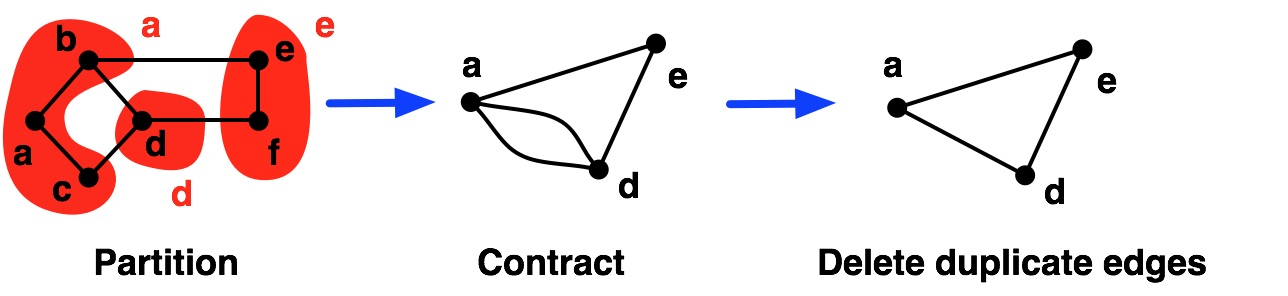
\includegraphics[width=5.0in]{./graph-contraction/media-introduction/contract-example5.jpg}
\end{center}

Contracting a graph down to a single vertex in three rounds:
\begin{center}
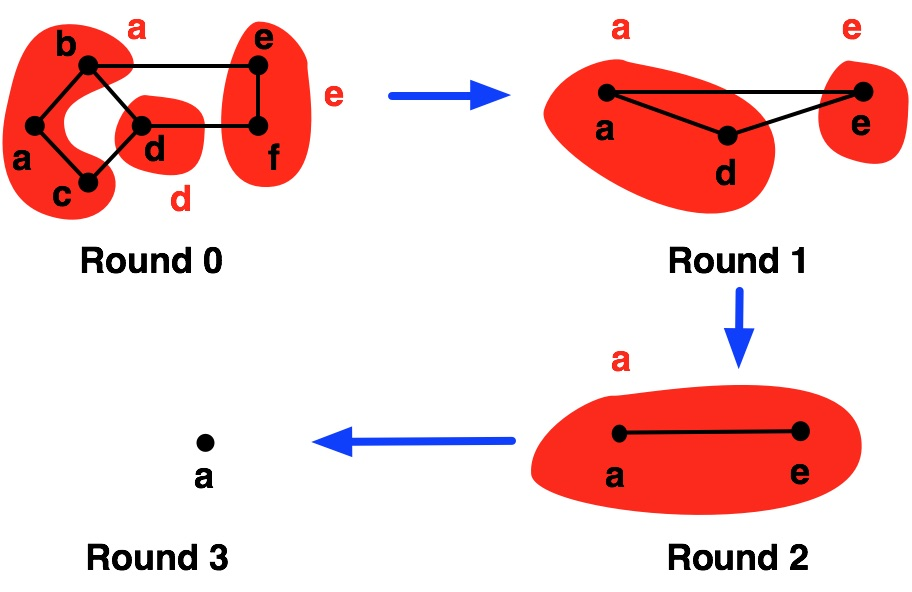
\includegraphics[width=4in]{./graph-contraction/media-introduction/graph-contraction-example-1.jpg}
\end{center}
\end{example}
\end{flex}

% \begin{simpleexample} [An example graph contraction]

%   An illustration of how we wish to apply graph contraction to solve
%   the connectivity problem.  In order to solve the problem, as we
%   contract the graph, we do not alter the connectivity of the
%   vertices: vertices that are not connected should not become
%   connected and vice versa.

% \begin{center}
% 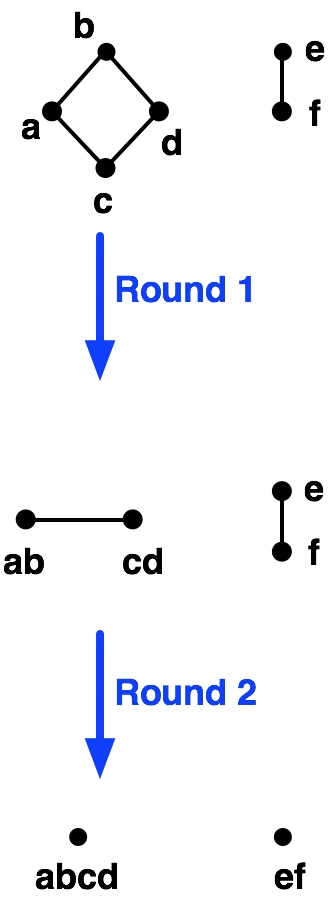
\includegraphics[width=1.5in]{./graph-contraction/media-introduction/contraction-example.jpg}
% \end{center}
% \end{simpleexample}


\begin{gram}[Construction of the Quotient Graph]
\label{graphcon::intro::graphcon::contruct-quotient}
To construct a quotient graph, we represent each block in the
partition with a vertex,
%
which we call a~\defn{super-vertex}.
%
We then ``map'' the edges of the graph to the quotient graph.
% 
Consider each edge $(u,v)$ in the graph.
%
\begin{itemize}
\item If the edge is an internal edge, then we skip the edge.

\item If the edge is a cut edge, then  we create a new edge between the
  super-vertices representing the blocks containing $u$ and $v$.
%
\end{itemize}

Because there can be many cut edges between two blocks, this approach may create
multiple edges between two super-vertices. 
%
We may remove duplicate edges or leave them in the graph, in which case we would be working with multigraphs. 
%
Either approach has its benefits and may, depending on the application, be preferable over the other.
\end{gram}

\begin{important}
\label{graphcon::intro::graphcon::disjointness}
Graph contraction is guided by a graph partition, which leads to blocks whose vertices are disjoint.
%
During the construction of the quotient graph, each vertex in the
graph is therefore mapped to a unique vertex in the quotient graph.
\end{important}


\begin{gram}[Applying Graph Contraction]
\label{graphcon::intro::graphcon::apply}
The ultimate goal of graph contraction technique is to reduce the size
of the graph by a constant fraction (possibly in expectation) at each
round of contraction.
%
Depending on the graphs of interest many different graph-partition
techniques can be used to achieve this goal.
%
As described, the graph-contraction technique is generic in
the kind of graph partition used.
%
In the following chapters on
%
\href{ch:graphcon::edge}{Edge Contraction}
%
and
%
\href{ch:graphcon::star}{Star Contraction}
%
we consider two techniques, edge partitioning and star partitioning,
and the resulting graph-contraction algorithms.
%
\end{gram}

